\clearpage

\section{Action Tree structure}
\label{sec:action_tree}

%\begin{figure*}[ht!]
%    \centering
%     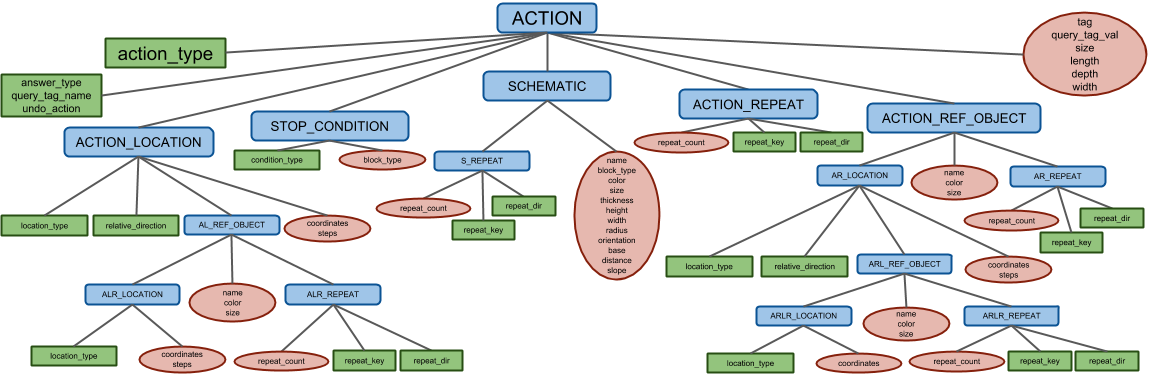
\includegraphics[natwidth=\linewidth]{figures/ActionGrammar.png}
%    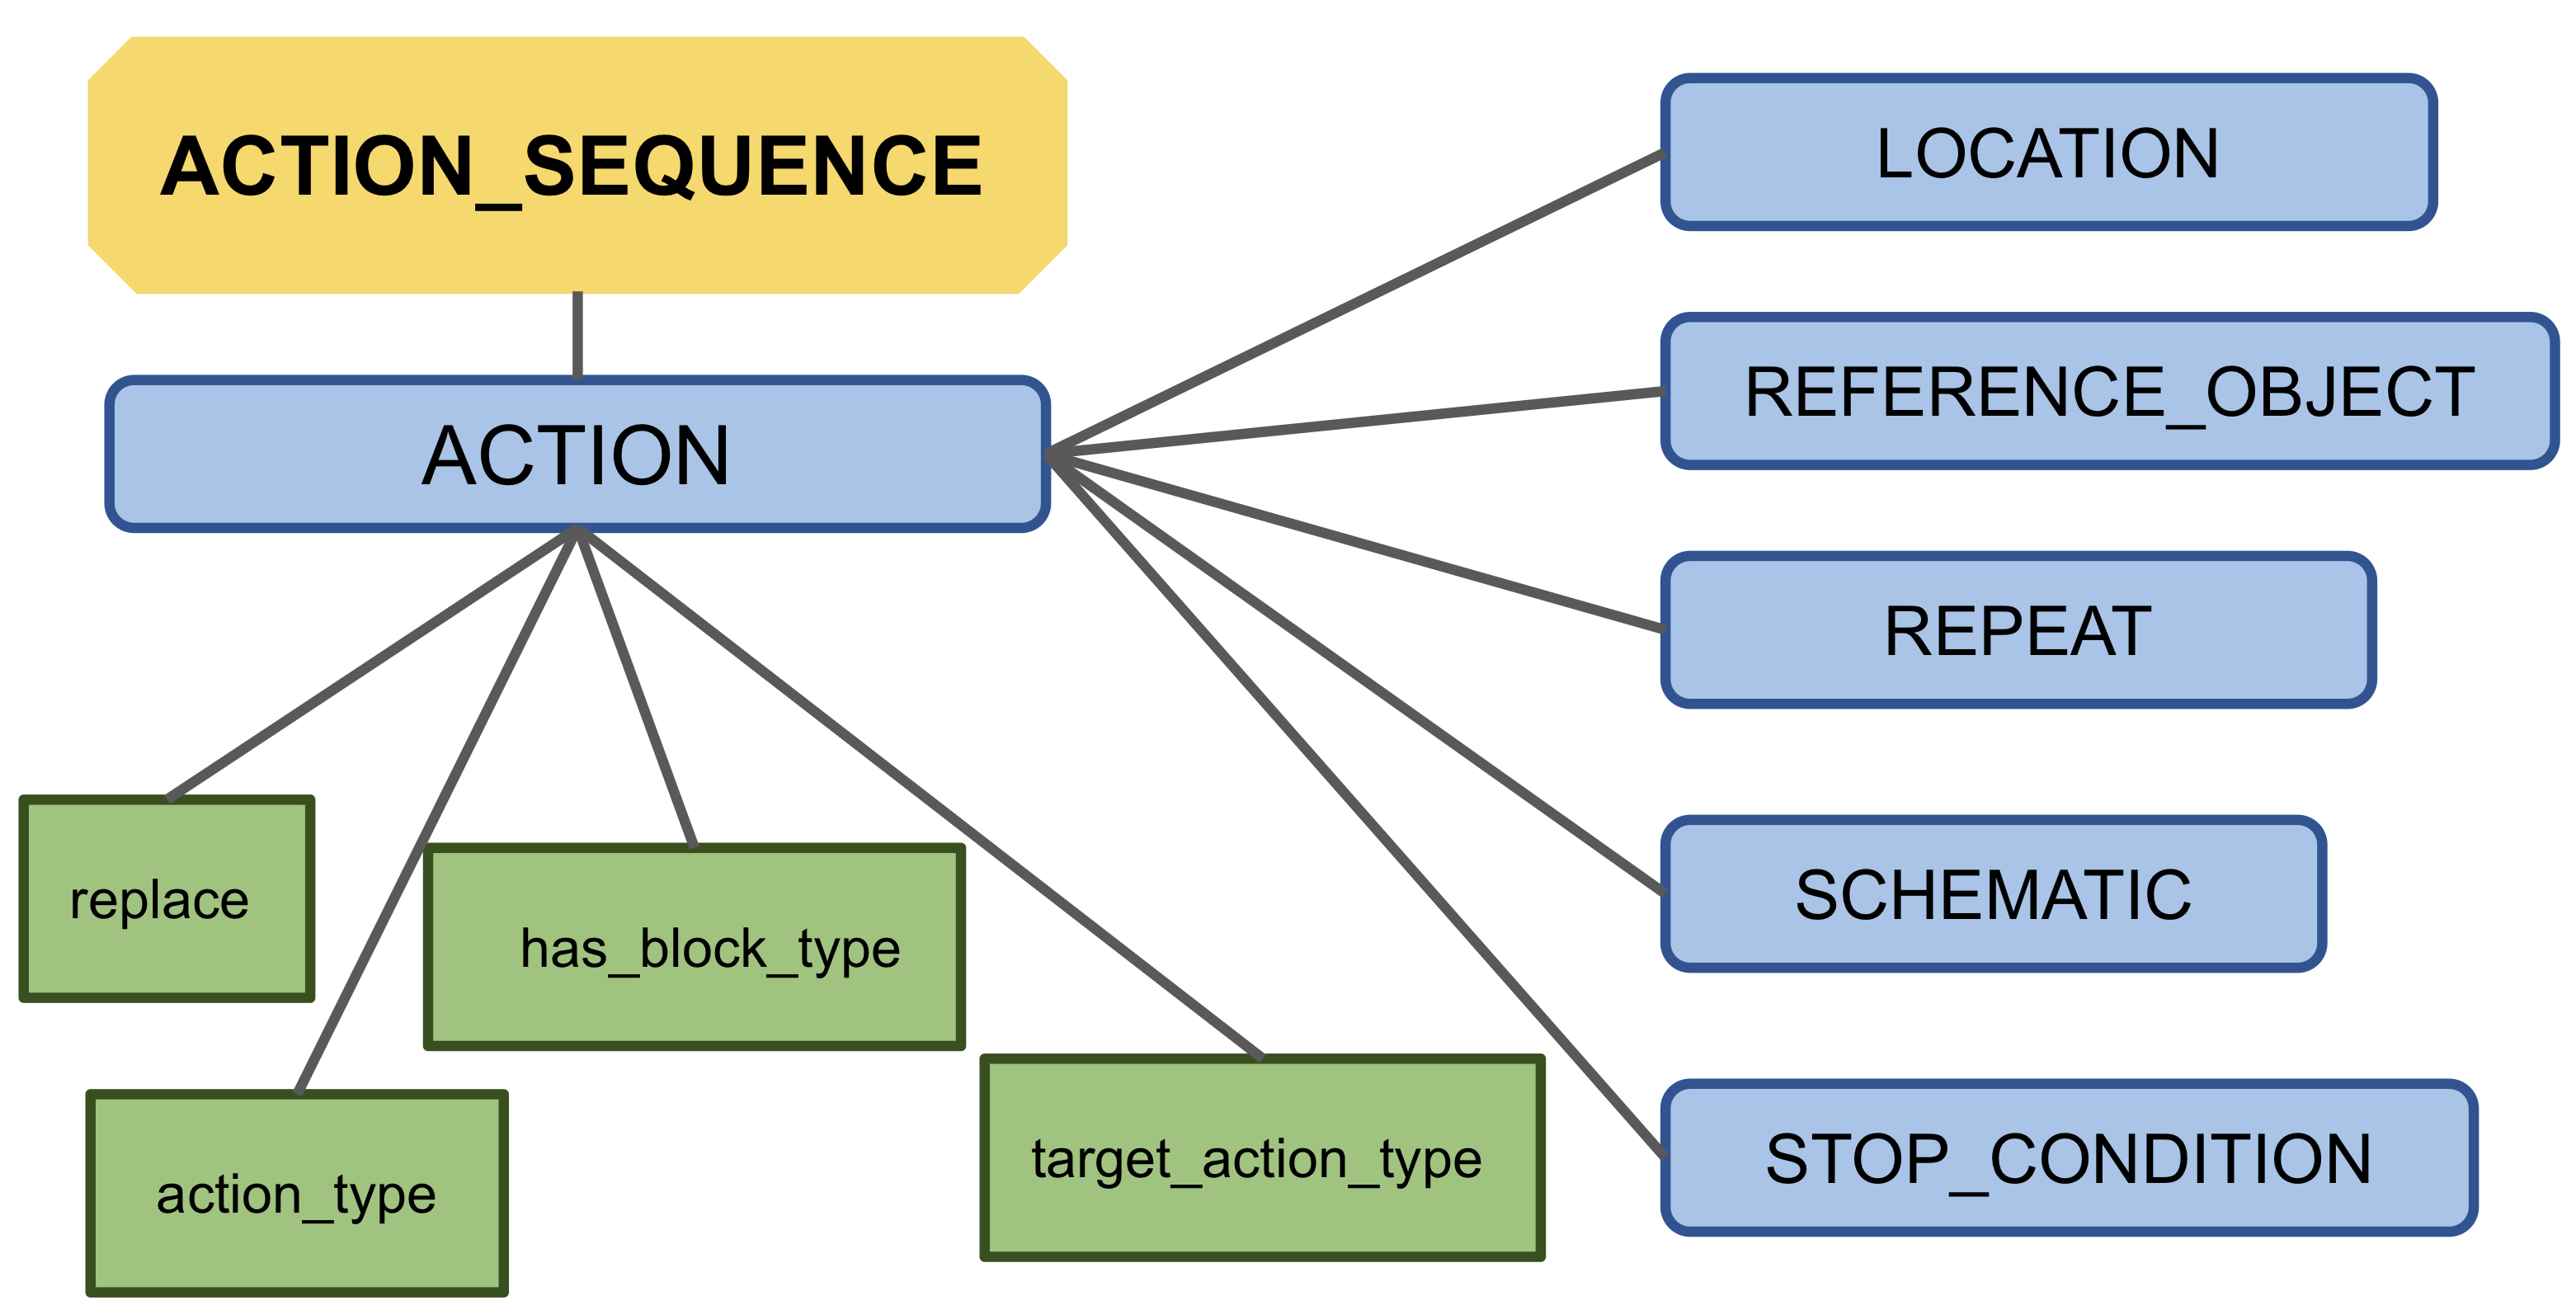
\includegraphics[width=0.70\linewidth]{figures/AS.png}
%    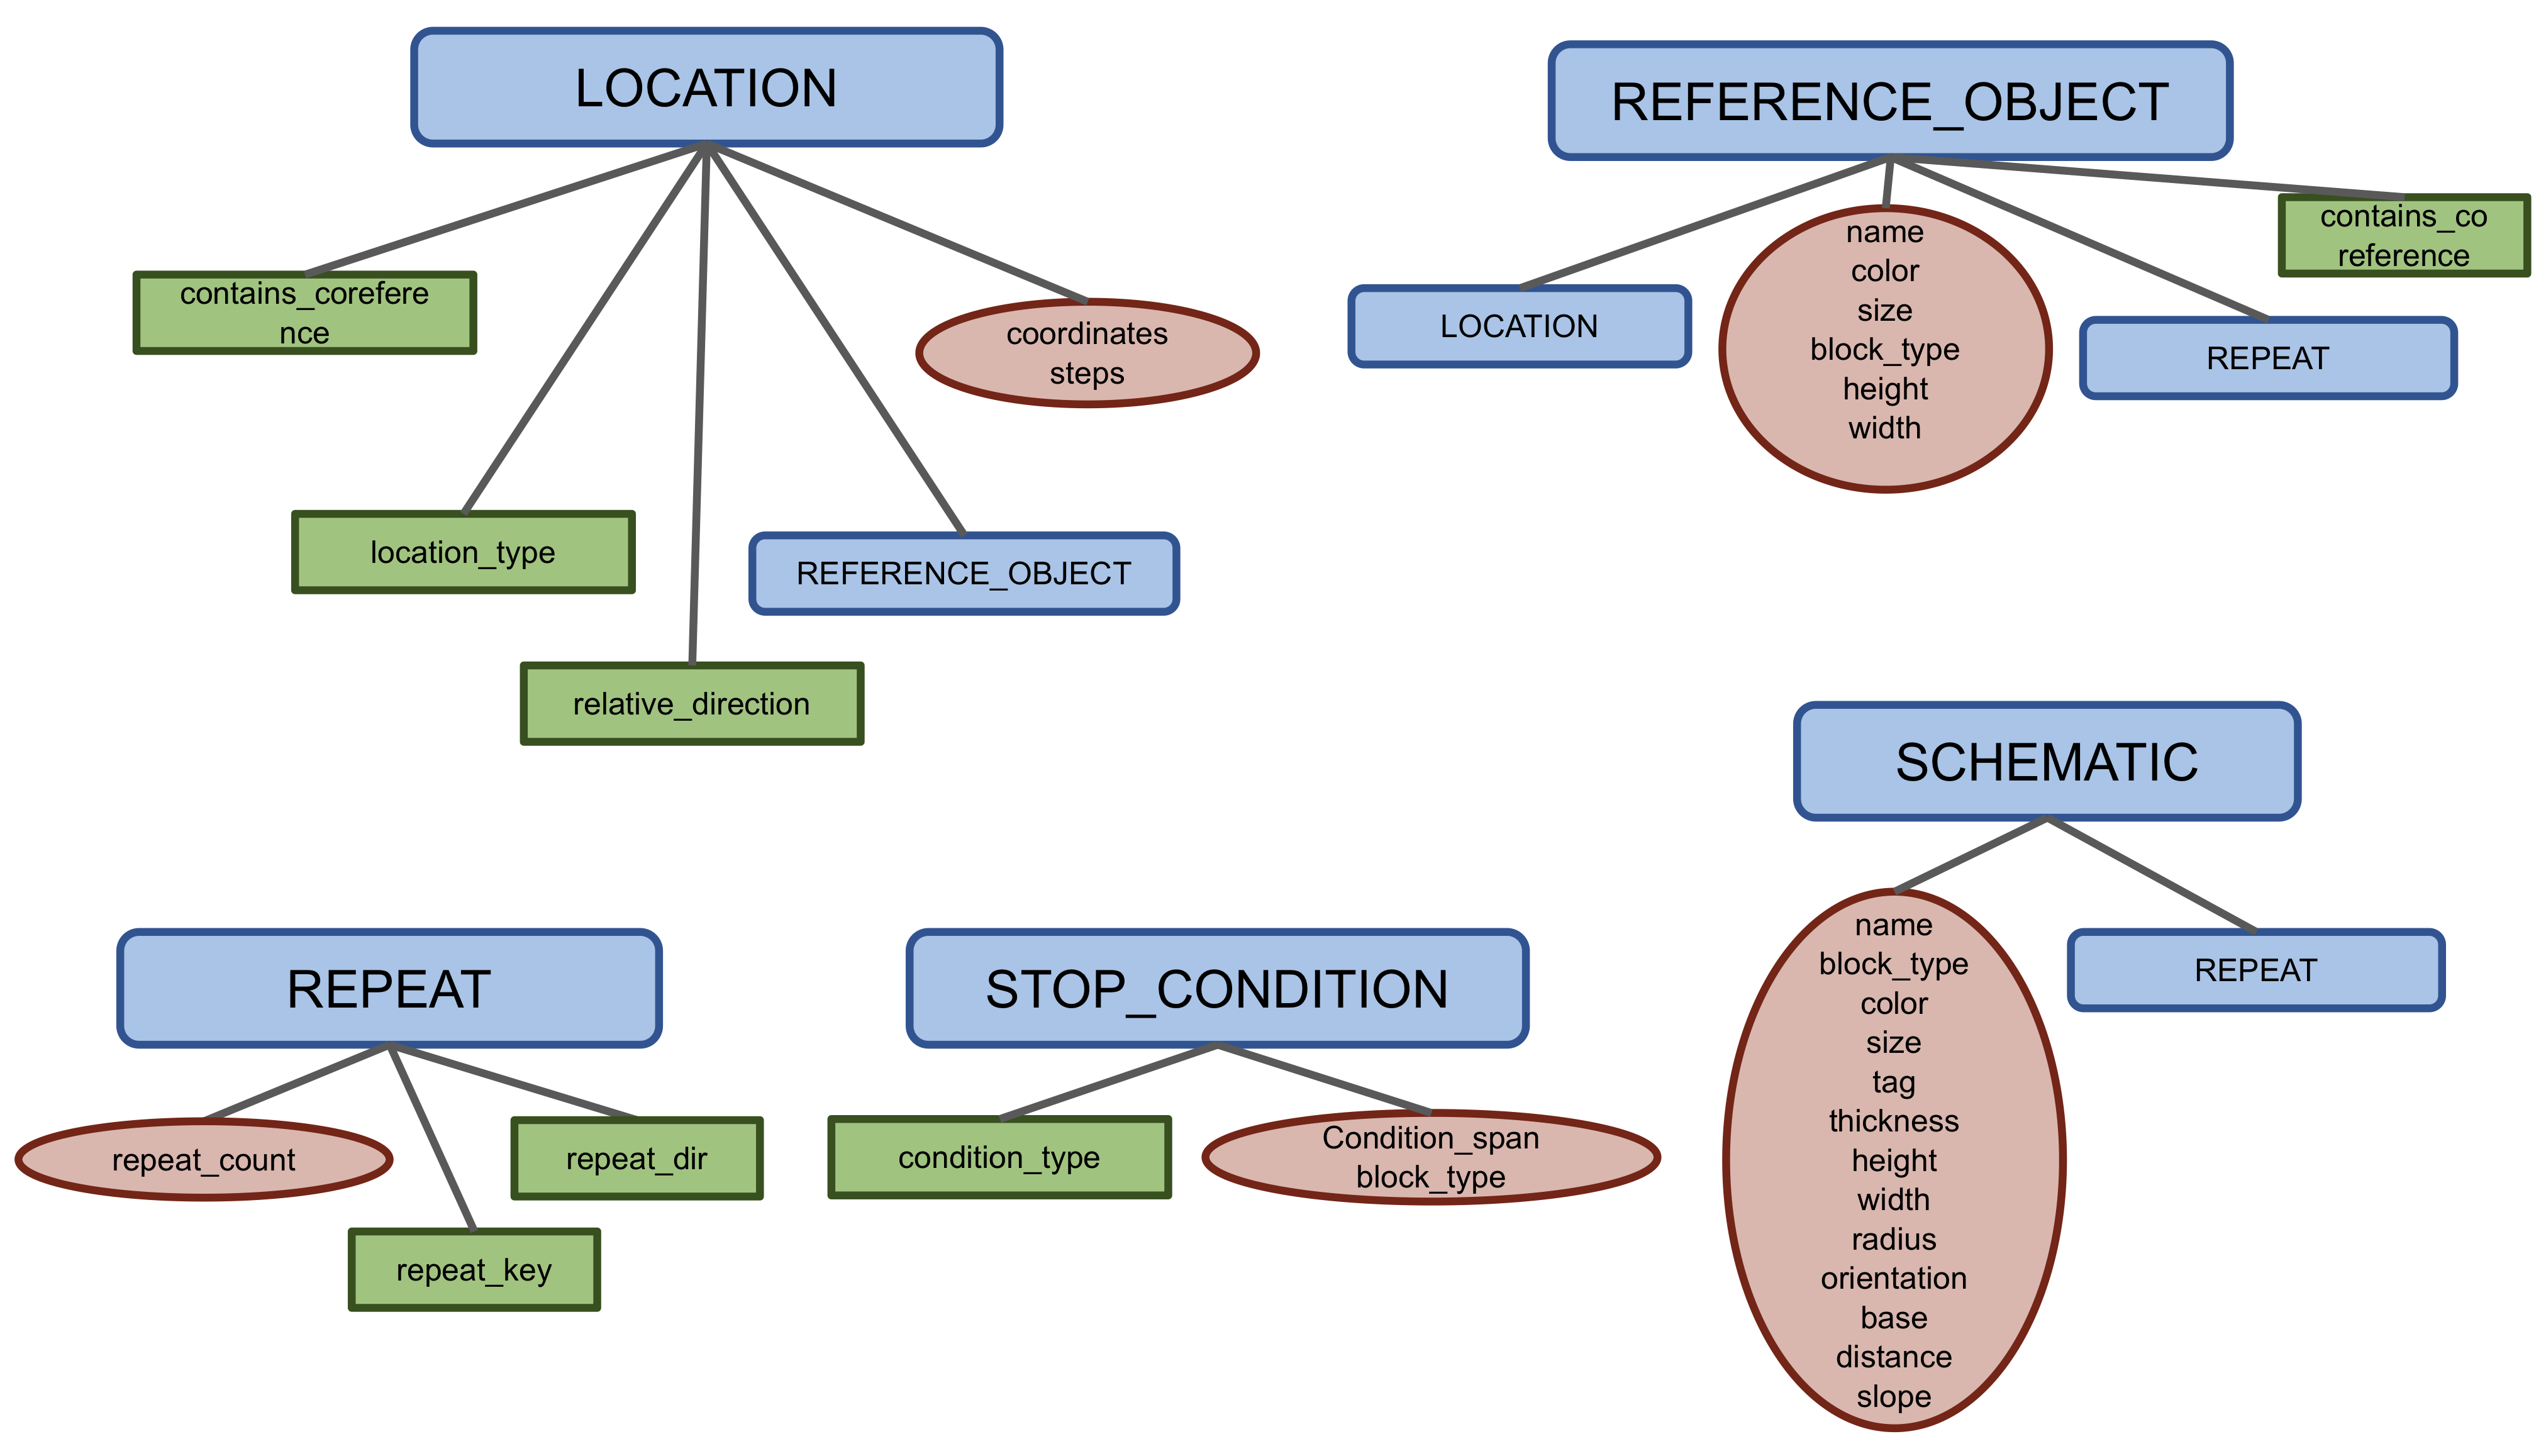
\includegraphics[width=0.30\linewidth]{figures/NOT_AS.png}
%    \caption{Action space grammar}
%    \label{fig:action_grammar}
%\end{figure*}
This section describes the details of logical form of each action.
We support three dialogue types: HUMAN\_GIVE\_COMMAND, GET\_MEMORY and PUT\_MEMORY.
The logical form for actions has been pictorially represented in Figures: \ref{fig:AS} and \ref{fig:NOT_AS}

We support the following actions in our dataset : Build, Copy, Dance, Spawn, Resume, Fill, Destroy, Move, Undo, Stop, Dig and FreeBuild.
A lot of the actions use  ``location'' and ``reference\_object'' as children in their logical forms. To make the logical forms more presentable, we have shown the detailed representation of a ``reference\_object'' (reused in action trees using the variable: ``REF\_OBJECT'') in Figure \ref{fig:ref_obj} and the representation of ``location'' (reused in action trees using the variable: ``LOCATION'') in figure \ref{fig:location}. The representations of actions refer to these variable names in their trees.


\begin{figure}[ht]
    \centering
    \fontsize{7pt}{8pt}\selectfont
    \begin{verbatim}
REF_OBJECT :
The recursion depth of REF_OBJECT in LOCATION 
was never greater than 1 in the data. So a REF_OBJECT
can have a LOCATION that has a REF_OBJECT that has a 
LOCATION (and the final location will be one of : 
COORDINATES / AGENT_POS / SPEAKER_POS / SPEAKER_LOOK).

"reference_object" : {
 "repeat" : {
  "repeat_key" : 'FOR' / 'ALL',
  "repeat_count" : span,
   "repeat_dir" : 'LEFT' / 'RIGHT' / 'UP'/ 
      'DOWN' / 'FRONT' / 'BACK' / 'AROUND'}
  "has_name" : span,
  "has_colour" : span,
  "has_size" : span,
  "has_tag": span,
  "has_length": span,
  "has_width": span,
  "has_height": span,
  "contains_coreference" : "yes",
  LOCATION  }
    \end{verbatim}
    \vspace{-20pt}
    \caption{Logical form of a reference\_object child}
    \vspace{-8pt}
    \label{fig:ref_obj}
\end{figure}


\begin{figure}[ht]
    \centering
    \fontsize{7pt}{8pt}\selectfont
    \begin{verbatim}
LOCATION:

"location" : {
 "location_type" : COORDINATES / REFERENCE_OBJECT / 
    AGENT_POS / SPEAKER_POS / SPEAKER_LOOK
 "steps" : span,
 "contains_coreference" : "yes",
 "relative_direction" : 'LEFT' / 'RIGHT' / 'UP'/ 
      'DOWN' / 'FRONT' / 'BACK' / 'AWAY' / 'INSIDE'
      / 'NEAR' / 'OUTSIDE' / 'BETWEEN',
 "coordinates" : span, (present if "location_type" is
   'COORDINATES),
  REF_OBJECT (present if "location_type" is 
   'REFERENCE_OBJECT')
 }
    \end{verbatim}
    \vspace{-20pt}
    \caption{Logical form of a location child}
    \vspace{-8pt}
    \label{fig:location}
\end{figure}


The detailed action tree for each action and dialogue type has been presented in the following subsections. Figure~\ref{fig:action_tree_ex} shows an example for a \textsc{build} action.

\begin{figure}[ht]
    \centering
    \small
    \begin{verbatim}
  0     1    2   3     4    5   6
"Make three oak wood houses to the
 7   8   9   10   11    12
left of the dark grey church."


{"dialogue_type" : "HUMAN_GIVE_COMMAND",
 "action_sequence" : [
   {
    "action_type" : "BUILD",
    "schematic": {
      "has_block_type": [0, [2, 3]],
      "has_name": [0, [4, 4]],
      "repeat": {
        "repeat_key": "FOR",
        "repeat_count": [1, 1]
      }},
     "location": {
       "relative_direction": "LEFT",
       "location_type": "REFERENCE_OBJECT",
       "reference_object": {
         "has_colour_": [0, [10, 11]],
         "has_name_": [0, [12, 12]] }
}}]}
    \end{verbatim}
    \vspace{-20pt}
    \caption{An example logical form. The spans are indexed as : [sentence\_number, [starting\_word\_index, ending\_word\_index]].  sentence\_number is 0 for the most recent sentence spoken in a dialogue and is 0 in our dataset since we support one-turn dialogues as of now.}
    \vspace{-8pt}
    \label{fig:action_tree_ex}
\end{figure}


\subsection{ Build Action}
This is the action to Build a schematic at an optional location. The Build logical form is shown in \ref{fig:build_dict} .


\begin{figure}[ht]
    \centering
    \fontsize{8pt}{8pt}\selectfont
    \begin{verbatim}
{ "dialogue_type" :  'HUMAN_GIVE_COMMAND',
 "action_sequence" : [
   {"action_type" :  'BUILD',
    LOCATION,
    "schematic" : {
      "repeat" : {
       "repeat_key" : 'FOR' / 'ALL',
       "repeat_count" : span,
       "repeat_dir" : 'LEFT' / 'RIGHT' / 'UP'/ 
          'DOWN' / 'FRONT' / 'BACK' / 'AROUND'}
      "has_name" : span,
      "has_block_type" : span,
      "has_size" : span,
      "has_orientation" : span,
      "has_thickness" : span,
      "has_colour" : span,
      "has_length": span,
      "has_height" : span,
      "has_radius" : span,
      "has_slope" : span,
      "has_width": span,
      "has_base" : span,
      "has_distance" : span,
     },
    "repeat" : {
      "repeat_key" : 'FOR' / 'ALL',
       "repeat_count" : span,
       "repeat_dir" : 'LEFT' / 'RIGHT' / 'UP'/ 
          'DOWN' / 'FRONT' / 'BACK' / 'AROUND'}
     } ] }
    \end{verbatim}
    \vspace{-20pt}
    \caption{Details of logical form for Build}
    \vspace{-8pt}
    \label{fig:build_dict}
\end{figure}


\subsection{Copy Action}
This is the action to copy a block object to an optional location. The copy action is represented as a "Build" with an optional "reference object" . The logical form  is shown in \ref{fig:copy_dict}.


\begin{figure}[ht]
    \centering
    \fontsize{8pt}{8pt}\selectfont
    \begin{verbatim}
{ "dialogue_type" :  'HUMAN_GIVE_COMMAND',
 "action_sequence" : [
   {"action_type" :  'BUILD',
    LOCATION,
    REF_OBJ,
    "repeat" : {
      "repeat_key" : 'FOR' / 'ALL',
       "repeat_count" : span,
       "repeat_dir" : 'LEFT' / 'RIGHT' / 'UP'/ 
          'DOWN' / 'FRONT' / 'BACK' / 'AROUND'}
     } ] }
    \end{verbatim}
    \vspace{-20pt}
    \caption{Details of logical form for Copy}
    \vspace{-8pt}
    \label{fig:copy_dict}
\end{figure}

\subsection{ Spawn Action}
This action indicates that the specified object should be spawned in the environment. The logical form is shown in: \ref{fig:spawn_dict}

\begin{figure}[ht]
    \centering
    \fontsize{8pt}{8pt}\selectfont
    \begin{verbatim}
{ "dialogue_type" :  'HUMAN_GIVE_COMMAND',
 "action_sequence" : [
   {"action_type" :  'SPAWN',
    LOCATION,
    REF_OBJ } ] }
    \end{verbatim}
    \vspace{-20pt}
    \caption{Details of logical form for Spawn action}
    \vspace{-8pt}
    \label{fig:spawn_dict}
\end{figure}



\subsection{ Fill Action}
This action states that a hole / negative shape at an optional location needs to be filled up. The logical form  is explained in : \ref{fig:fill_dict}

\begin{figure}[ht]
    \centering
    \fontsize{8pt}{8pt}\selectfont
    \begin{verbatim}
{ "dialogue_type" :  'HUMAN_GIVE_COMMAND',
 "action_sequence" : [
   {"action_type" :  'FILL',
    "has_block_type" : span,
    REF_OBJ } ] }
    \end{verbatim}
    \vspace{-20pt}
    \caption{Details of logical form  for Fill}
    \vspace{-8pt}
    \label{fig:fill_dict}
\end{figure}



\subsection{ Destroy Action}
This action indicates the intent to destroy a block object at an optional location. The logical form  is shown in: \ref{fig:destroy_dict}

Destroy action can have one of the following as the child:
\begin{itemize}
	\setlength\itemsep{0.0em}
	\item reference object
	\item nothing
\end{itemize}

\begin{figure}[ht]
    \centering
    \fontsize{8pt}{8pt}\selectfont
    \begin{verbatim}
{ "dialogue_type" :  'HUMAN_GIVE_COMMAND',
 "action_sequence" : [
   {"action_type" :  'DESTROY',
    REF_OBJ } ] }
    \end{verbatim}
    \vspace{-20pt}
    \caption{Details of logical form  Destroy}
    \vspace{-8pt}
    \label{fig:destroy_dict}
\end{figure}



\subsection{Move Action}
This action states that the agent should move to the specified location, the corresponding logical form  is in: \ref{fig:move_dict}

Move action can have one of the following as its child:
\begin{itemize}
	\setlength\itemsep{0.0em}
	\item location
	\item stop condition (stop moving when a condition is met)
	\item location and stop condition
	\item neither
\end{itemize}


\begin{figure}[ht]
    \centering
    \fontsize{8pt}{8pt}\selectfont
    \begin{verbatim}
{ "dialogue_type" :  'HUMAN_GIVE_COMMAND',
 "action_sequence" : [
   {"action_type" :  'MOVE',
    LOCATION,
    "stop_condition" : {
     "condition_type": 'ADJACENT_TO_BLOCK_TYPE' /
           'NEVER',
     "block_type": span,
     "condition_span" :  span },
    "repeat" : {
      "repeat_key" : 'FOR' / 'ALL',
       "repeat_count" : span,
       "repeat_dir" : 'LEFT' / 'RIGHT' / 'UP'/ 
          'DOWN' / 'FRONT' / 'BACK' / 'AROUND'}
     } ] }

    \end{verbatim}
    \vspace{-20pt}
    \caption{Details of logical form  for Move action}
    \vspace{-8pt}
    \label{fig:move_dict}
\end{figure}

\subsection{ Dig Action}
This action represents the intent to dig a hole / negative shape of optional dimensions at an optional location. The logical form is in \ref{fig:dig_dict}

\begin{figure}[ht]
    \centering
    \fontsize{8pt}{8pt}\selectfont
    \begin{verbatim}
{ "dialogue_type" :  'HUMAN_GIVE_COMMAND',
 "action_sequence" : [
   {"action_type" :  'DIG',
    LOCATION,
    "schematic" : {
       "repeat" : {
         "repeat_key" : 'FOR' / 'ALL',
         "repeat_count" : span,
         "repeat_dir" : 'LEFT' / 'RIGHT' / 'UP'/ 
          'DOWN' / 'FRONT' / 'BACK' / 'AROUND'}
      "has_size" : span,
      "has_length": span,
      "has_depth" :  span,
      "has_width" :  span
       },
    "stop_condition" : {
      "condition_type" : 'ADJACENT_TO_BLOCK_TYPE' /
           'NEVER',
      "block_type": span }
     } ] }
    \end{verbatim}
    \vspace{-20pt}
    \caption{Details of logical form  for Dig action}
    \vspace{-8pt}
    \label{fig:dig_dict}
\end{figure}


\subsection{Dance Action}
This action represents that the agent performs a movement of a certain kind. Note that this action is different than a Move action in that the path or step-sequence here is more important than the destination. The logical form is shown in \ref{fig:dance_dict}

\begin{figure}[ht]
    \centering
    \fontsize{8pt}{8pt}\selectfont
    \begin{verbatim}
{ "dialogue_type" :  'HUMAN_GIVE_COMMAND',
 "action_sequence" : [
   {"action_type" :  'DANCE',
    LOCATION,
    "stop_condition" : {
      "condition_type" : 'NEVER'}
    "repeat: {
      "repeat_key" : FOR,
      "repeat_count" :  span }
     } ] }
    \end{verbatim}
    \vspace{-20pt}
    \caption{Details of logical form for Dance action}
    \vspace{-8pt}
    \label{fig:dance_dict}
\end{figure}

\subsection{FreeBuild Action}
This action represents that the agent should complete an already existing half-finished block object, using its mental model. The logical form is explained in: \ref{fig:freebuild_dict}

FreeBuild action can have one of the following as its child:
\begin{itemize}
	\setlength\itemsep{0.0em}
	\item reference object only
	\item reference object and location
\end{itemize}


\begin{figure}[ht]
    \centering
    \fontsize{8pt}{8pt}\selectfont
    \begin{verbatim}
{ "dialogue_type" :  'HUMAN_GIVE_COMMAND',
 "action_sequence" : [
   {"action_type" :  'FREEBUILD',
    REF_OBJECT,
    LOCATION }  ]  }
    \end{verbatim}
    \vspace{-20pt}
    \caption{Details of logical form for Freebuild action}
    \vspace{-8pt}
    \label{fig:freebuild_dict}
\end{figure}


\subsection{ Undo Action}
This action states the intent to revert the specified action, if any. The logical form is in \ref{fig:undo_dict}.
Undo action can have on of the following as its child:
\begin{itemize}
	\setlength\itemsep{0.0em}
	\item target\_action\_type 
	\item nothing (meaning : undo the last action)
\end{itemize}

\begin{figure}[ht]
    \centering
    \fontsize{8pt}{8pt}\selectfont
    \begin{verbatim}
{ "dialogue_type" :  'HUMAN_GIVE_COMMAND',
 "action_sequence" : [
   {"action_type" :  'UNDO',
    "target_action_type" : span } ] }
    \end{verbatim}
    \vspace{-20pt}
    \caption{Details of logical form for Undo action}
    \vspace{-8pt}
    \label{fig:undo_dict}
\end{figure}


\subsection{ Stop Action}
This action indicates stop and the logical form is shown in \ref{fig:stop_dict}

\begin{figure}[ht]
    \centering
    \fontsize{8pt}{8pt}\selectfont
    \begin{verbatim}
{ "dialogue_type" :  'HUMAN_GIVE_COMMAND',
 "action_sequence" : [
   {"action_type" :  'STOP',
    "target_action_type" : span } ] }
    \end{verbatim}
    \vspace{-20pt}
    \caption{Details of logical form for Stop action}
    \vspace{-8pt}
    \label{fig:stop_dict}
\end{figure}

\subsection{Resume Action}
This action indicates that the previous action should be resumed, the logical form is shown in: \ref{fig:resume_dict}

\begin{figure}[ht]
    \centering
    \fontsize{8pt}{8pt}\selectfont
    \begin{verbatim}
{ "dialogue_type" :  'HUMAN_GIVE_COMMAND',
 "action_sequence" : [
   {"action_type" :  'RESUME',
    "target_action_type" : span } ] }
    \end{verbatim}
    \vspace{-20pt}
    \caption{Details of logical form for Resume action}
    \vspace{-8pt}
    \label{fig:resume_dict}
\end{figure}

\subsection{Get Memory Dialogue type}
This dialogue type represents the agent answering a question about the environment.
This is similar to the setup in Visual Question Answering. The logical form is represented in: \ref{fig:answer_dict}

Get Memory dialogue has the following as its children: filters, answer type and tag name.
This dialogue type represents the type of expected answer : counting, querying a specific attribute or querying everything ("what is the size of X" vs "what is X" )

\begin{figure}[ht]
    \centering
   \fontsize{8pt}{8pt}\selectfont
    
    \begin{verbatim}
{ "dialogue_type": "GET_MEMORY",
  "filters": {
    "temporal": CURRENT,
    "type": "ACTION" / "AGENT" / "REFERENCE_OBJECT",
    "action_type": BUILD / DESTROY / DIG / FILL / 
         SPAWN / MOVE
    "reference_object" : {
      LOCATION,
      "has_size" : span,
      "has_colour" : span,
      "has_name" : span,
      "coref_resolve": span,
      },
    },
  "answer_type": "TAG" / "EXISTS" ,
  "tag_name" : 'has_name' / 'has_size' /'has_colour' / 
        'action_name' / 'action_reference_object_name' / 
        'move_target' / 'location' ,
  "replace": true
}
    \end{verbatim}
    \vspace{-20pt}
    \caption{Details of logical form for Get Memory Dialogue}
    \vspace{-8pt}
    \label{fig:answer_dict}
\end{figure}


\subsection{Put Memory Dialogue}
This dialogue type represents that a reference object should be tagged with the given tag and the logical form is shown in: \ref{fig:tag_dict}


\begin{figure}[ht]
    \centering
    \fontsize{8pt}{8pt}\selectfont
    \begin{verbatim}
{ "dialogue_type": "PUT_MEMORY",
  "filters": { REF_OBJECT },
  "upsert" : {
      "memory_data": {
        "memory_type": "REWARD" / "TRIPLE",
        "reward_value": "POSITIVE" / "NEGATIVE",
        "has_tag" : span,
        "has_colour": span,
        "has_size": span
      } } }
    \end{verbatim}
    \vspace{-20pt}
    \caption{Details of logical form for Put Memory Dialogue}
    \vspace{-8pt}
    \label{fig:tag_dict}
\end{figure}



\subsection{ Noop Dialogue}
This dialogue type indicates no operation should be performed, the logical form is shown in : \ref{fig:noop_dict}

\begin{figure}[ht]
    \centering
    \fontsize{8pt}{8pt}\selectfont
    \begin{verbatim}
{ "dialogue_type": "NOOP" }
    \end{verbatim}
    \vspace{-20pt}
    \caption{Details of logical form for Noop Dialogue}
    \vspace{-8pt}
    \label{fig:noop_dict}
\end{figure}
